\documentclass[11pt]{article}

\usepackage[a4paper,margin=1in]{geometry}
\usepackage[T1]{fontenc}
\usepackage[utf8]{inputenc}
\usepackage{lmodern}
\usepackage{microtype}
\usepackage{amsmath,amssymb}
\usepackage{booktabs}
\usepackage{csquotes}
\usepackage{graphicx}
\usepackage{tikz}
\usepackage[hidelinks]{hyperref}
\usepackage[nameinlink,capitalise]{cleveref}

\title{An eigenvalue-weighted extension of branch saturation testing}
\author{Berk Sakalli}
\date{\today}

\begin{document}
\maketitle

\begin{abstract}
Branch saturation tests ask whether two subtrees connected by a branch still share phylogenetic signal. SatuTe answers this question with a coherence coefficient for the dominant non-stationary eigenvalue of a reversible substitution model. This draft defines an eigenvalue-weighted extension that keeps the same subtree likelihood notation and null test, but replaces a single coefficient by a branch-length-aware sum over non-stationary coherence coefficients. The extension is identical to SatuTe under Jukes--Cantor symmetry and gives a paired general time-reversible comparison in which eigenvectors describe directions of signal and eigenvalues determine the expected persistence of those directions.
\end{abstract}

Saturation is a practical failure mode for phylogenomic inference. A branch can be present in a maximum-likelihood tree, and can even have high conventional support, while the alignment no longer contains information that reliably connects the two subtrees separated by that branch. SatuTe formalized this problem as a branch-specific test of subtree independence: for a branch \(AB\), the subtrees \(T_A\) and \(T_B\) are treated as phylogenetically informative if their subpatterns \(\partial_A\) and \(\partial_B\) show shared signal beyond what is expected under independent evolution \cite{manuel2025satute}. This reframes saturation from a pairwise sequence property into a testable property of a split in a tree.

The existing statistic uses the dominant non-stationary eigenspace. For a site pattern \(\partial\), SatuTe computes the partial likelihood vectors \(L(\partial_A)\) and \(L(\partial_B)\), the subtree pattern probabilities \(P(\partial_A)=\langle L(\partial_A),\pi\rangle\) and \(P(\partial_B)=\langle L(\partial_B),\pi\rangle\), and the coherence coefficient associated with the second largest eigenvalue of the rate matrix. With eigenvalues \(\lambda_0=0>\lambda_1\geq\lambda_2\geq\lambda_3\) and left eigenvectors \(h_i\), the published coefficient for a simple eigenvalue is
\begin{equation}
C_{\partial i}
=
\left\langle \frac{L(\partial_A)}{P(\partial_A)}, h_i \right\rangle
\left\langle \frac{L(\partial_B)}{P(\partial_B)}, h_i \right\rangle .
\label{eq-coherence}
\end{equation}
For the dominant non-stationary mode, the empirical statistic is \(\hat C_1=n^{-1}\sum_{s=1}^{n}C_{\partial_s 1}\), with variance estimator \(\hat\sigma_1^2\) and one-sided statistic \(Z=\sqrt{n}\hat C_1/\hat\sigma_1\). Rejecting \(Z\leq z_\alpha\) is not the aim; SatuTe rejects subtree independence when \(Z>z_\alpha\), and therefore calls branch \(AB\) phylogenetically informative. Failure to reject means that \(AB\) is treated as saturated.

This construction tests whether the dominant surviving spectral direction links \(T_A\) and \(T_B\). Under a general time-reversible (GTR) model, \(\lambda_1\), \(\lambda_2\) and \(\lambda_3\) are usually distinct. Their eigenvectors \(h_i\) describe different directions in nucleotide state space, while their eigenvalues describe different decay rates along branch \(AB\). A statistic that uses only \(C_{\partial 1}\) can omit signal carried by \(h_2\) or \(h_3\). A statistic that sums all \(C_{\partial i}\) equally treats rapidly decaying modes as if they persist over long branches. The weighted statistic tested here uses all non-stationary modes but scales them by their relative decay.

\begin{figure}[htbp]
  \centering
  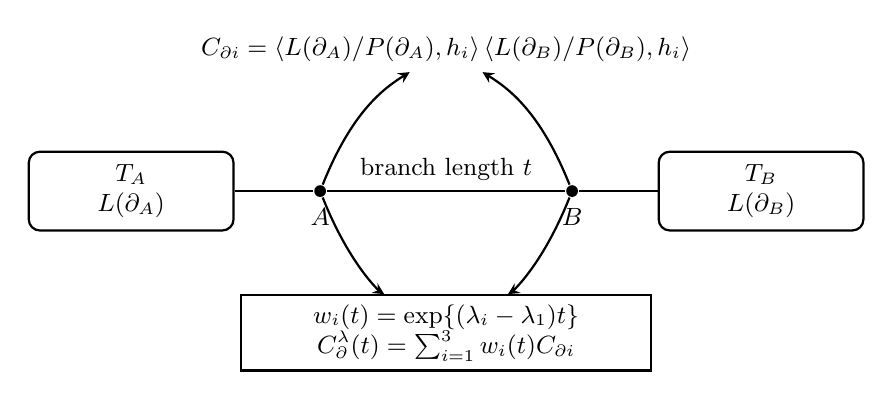
\begin{tikzpicture}[font=\small,>=stealth,thick]
    \node[draw,rounded corners,align=center,minimum width=2.6cm,minimum height=1.0cm] (ta) at (0,0) {\(T_A\)\\\(L(\partial_A)\)};
    \node[draw,rounded corners,align=center,minimum width=2.6cm,minimum height=1.0cm] (tb) at (8,0) {\(T_B\)\\\(L(\partial_B)\)};
    \node[circle,fill=black,inner sep=1.5pt,label=below:{\(A\)}] (a) at (2.4,0) {};
    \node[circle,fill=black,inner sep=1.5pt,label=below:{\(B\)}] (b) at (5.6,0) {};
    \draw (ta) -- (a);
    \draw (a) -- node[above]{branch length \(t\)} (b);
    \draw (b) -- (tb);
    \node[align=center] (coeff) at (4,1.8) {\(C_{\partial i}=
      \left\langle L(\partial_A)/P(\partial_A),h_i\right\rangle
      \left\langle L(\partial_B)/P(\partial_B),h_i\right\rangle\)};
    \draw[->] (a) .. controls (2.8,1.0) and (3.2,1.3) .. (coeff);
    \draw[->] (b) .. controls (5.2,1.0) and (4.8,1.3) .. (coeff);
    \node[draw,align=center,minimum width=5.2cm,minimum height=0.9cm] (weight) at (4,-1.8)
      {\(w_i(t)=\exp\{(\lambda_i-\lambda_1)t\}\)\\
       \(C_{\partial}^{\lambda}(t)=\sum_{i=1}^{3}w_i(t)C_{\partial i}\)};
    \draw[->] (a) .. controls (2.8,-1.0) and (3.2,-1.3) .. (weight);
    \draw[->] (b) .. controls (5.2,-1.0) and (4.8,-1.3) .. (weight);
  \end{tikzpicture}
  \caption{\textbf{Eigenvalue weighting in SatuTe notation.} Branch \(AB\) splits a site pattern \(\partial\) into \(\partial_A\) and \(\partial_B\). SatuTe computes coherence coefficients \(C_{\partial i}\) from normalized partial likelihood vectors and eigenvectors \(h_i\). The extension keeps these coefficients but weights each non-stationary mode by its relative persistence over branch length \(t\).}
\end{figure}

\section*{Results}

\subsection*{A weighted coefficient extends the SatuTe statistic}

The spectral decomposition used by SatuTe gives
\begin{equation}
\frac{P(\partial\mid t)}{P(\partial_A)P(\partial_B)}
=
1+\sum_{i=1}^{3} C_{\partial i}\exp(\lambda_i t).
\label{eq-central}
\end{equation}
Equation~\eqref{eq-central} contains both the coherence coefficients and their branch-length decay terms. The coefficient \(C_{\partial i}\) measures whether the two subtrees agree in the spectral direction \(h_i\). The term \(\exp(\lambda_i t)\) measures how much of that direction remains after evolution across branch \(AB\). Because all non-stationary eigenvalues are negative, the modes with more negative \(\lambda_i\) decay faster.

We define the eigenvalue-weighted coherence for pattern \(\partial\) as
\begin{equation}
C_{\partial}^{\lambda}(t)
=
\sum_{i=1}^{3} w_i(t)C_{\partial i},
\qquad
w_i(t)=\exp\{(\lambda_i-\lambda_1)t\}.
\label{eq-weighted-coherence}
\end{equation}
The relative weight \(w_i(t)\) sets \(w_1(t)=1\) and downweights modes that decay faster than the dominant non-stationary mode. This normalization keeps the published SatuTe coefficient as the reference scale while allowing additional eigenvectors to contribute when their expected persistence across branch \(AB\) is non-negligible.

For an alignment of \(n\) independently evolving sites, the empirical coefficient is
\begin{equation}
\hat C_{\lambda}(t)=\frac{1}{n}\sum_{s=1}^{n}C_{\partial_s}^{\lambda}(t).
\label{eq-weighted-mean}
\end{equation}
The variance estimator follows the same structure as the SatuTe estimator for a repeated second largest eigenvalue, but includes the mode weights:
\begin{equation}
\hat\sigma_{\lambda}^{2}(t)
=
\sum_{i=1}^{3}\sum_{j=1}^{3}
w_i(t)w_j(t)\hat\sigma_{A,i,j}^{2}\hat\sigma_{B,i,j}^{2}.
\label{eq-weighted-variance}
\end{equation}
The corresponding test statistic is
\begin{equation}
Z_{\lambda}(t)=\frac{\sqrt{n}\hat C_{\lambda}(t)}{\hat\sigma_{\lambda}(t)}.
\label{eq-weighted-z}
\end{equation}
The decision rule is unchanged: branch \(AB\) is called phylogenetically informative when \(Z_{\lambda}(t)>z_\alpha\), or when \(Z_{\lambda}(t)>z_{\alpha/(m_A m_B)}\) under the same Bonferroni correction used for maximum-likelihood tree double dipping.

\subsection*{The Jukes--Cantor case is unchanged}

The Jukes--Cantor (JC) model has one stationary eigenvalue and a three-dimensional non-stationary eigenspace with \(\lambda_1=\lambda_2=\lambda_3\). Therefore \(w_i(t)=1\) for all non-stationary modes in \cref{eq-weighted-coherence}. The weighted statistic becomes
\begin{equation}
C_{\partial}^{\lambda}(t)
=
\sum_{k=1}^{3} C_{\partial 1,k}
=
C_{\partial 1},
\label{eq-jc-collapse}
\end{equation}
which is the multiplicity-three expression used by SatuTe. Thus, the weighted statistic does not change the JC statistic. When the substitution model does not distinguish among the non-stationary directions, eigenvalue weighting does not introduce a distinction.

\subsection*{GTR separates direction from persistence}

Under a typical GTR model, the second largest eigenvalue has multiplicity one. The published statistic therefore uses \(C_{\partial 1}\), the most persistent non-stationary direction. This choice follows the slowest approach to stationarity. It can, however, discard signal in \(h_2\) and \(h_3\) when branch \(AB\) is short enough that those directions remain visible.

The unweighted all-mode alternative, \(C_{\partial}^{\mathrm{all}}=\sum_{i=1}^{3}C_{\partial i}\), can detect additional spectral agreement, but it does not account for different decay rates. The weighted statistic in \cref{eq-weighted-coherence} separates these two effects. For short branches, \(w_i(t)\) remains close to one and multiple directions can contribute. For long branches, \(w_i(t)\) approaches zero for faster modes and the statistic approaches the dominant SatuTe coefficient.

\subsection*{The original SatuTe simulations define the baseline}

The manuscript archive fixes the baseline simulation design more precisely than the article text alone. For the five-taxon simulation, the tested external branch \(AB\) connects taxon \(B\) to the root \(A\) of a balanced four-taxon subtree \(T_A\). All branches inside \(T_A\) have length 0.2, and the length of \(AB\) is varied. For the 16-taxon simulation, \(AB\) connects the roots \(A\) and \(B\) of two balanced eight-taxon subtrees. Branch lengths inside these subtrees are not fixed; external and internal branches are sampled from EvoNAPS-derived empirical branch-length distributions in the interval 0.04 to 0.2. In both cases, the branch length of \(AB\) is varied over the same 16-value grid, and 1,000 DNA alignments are generated for each combination of tree case, alignment length and branch length under the JC model with Seq-Gen.

The four analysis scenarios are also part of the statistical design, not merely plotting choices. Each simulated alignment is analyzed on the true tree with fixed true branch lengths, on the true topology with maximum-likelihood branch lengths, on a maximum-likelihood inferred tree, and on the same maximum-likelihood tree with a Bonferroni-corrected threshold. The correction is \(\alpha/4\) for the five-taxon external branch and \(\alpha/64\) for the 16-taxon internal branch. In the original 16-taxon analysis, maximum-likelihood trees that failed to recover the split induced by \(AB\) were discarded before the fraction of informative instances was computed. This discard rule must be preserved in any direct comparison to the published curves.

\begin{figure}[htbp]
  \centering
  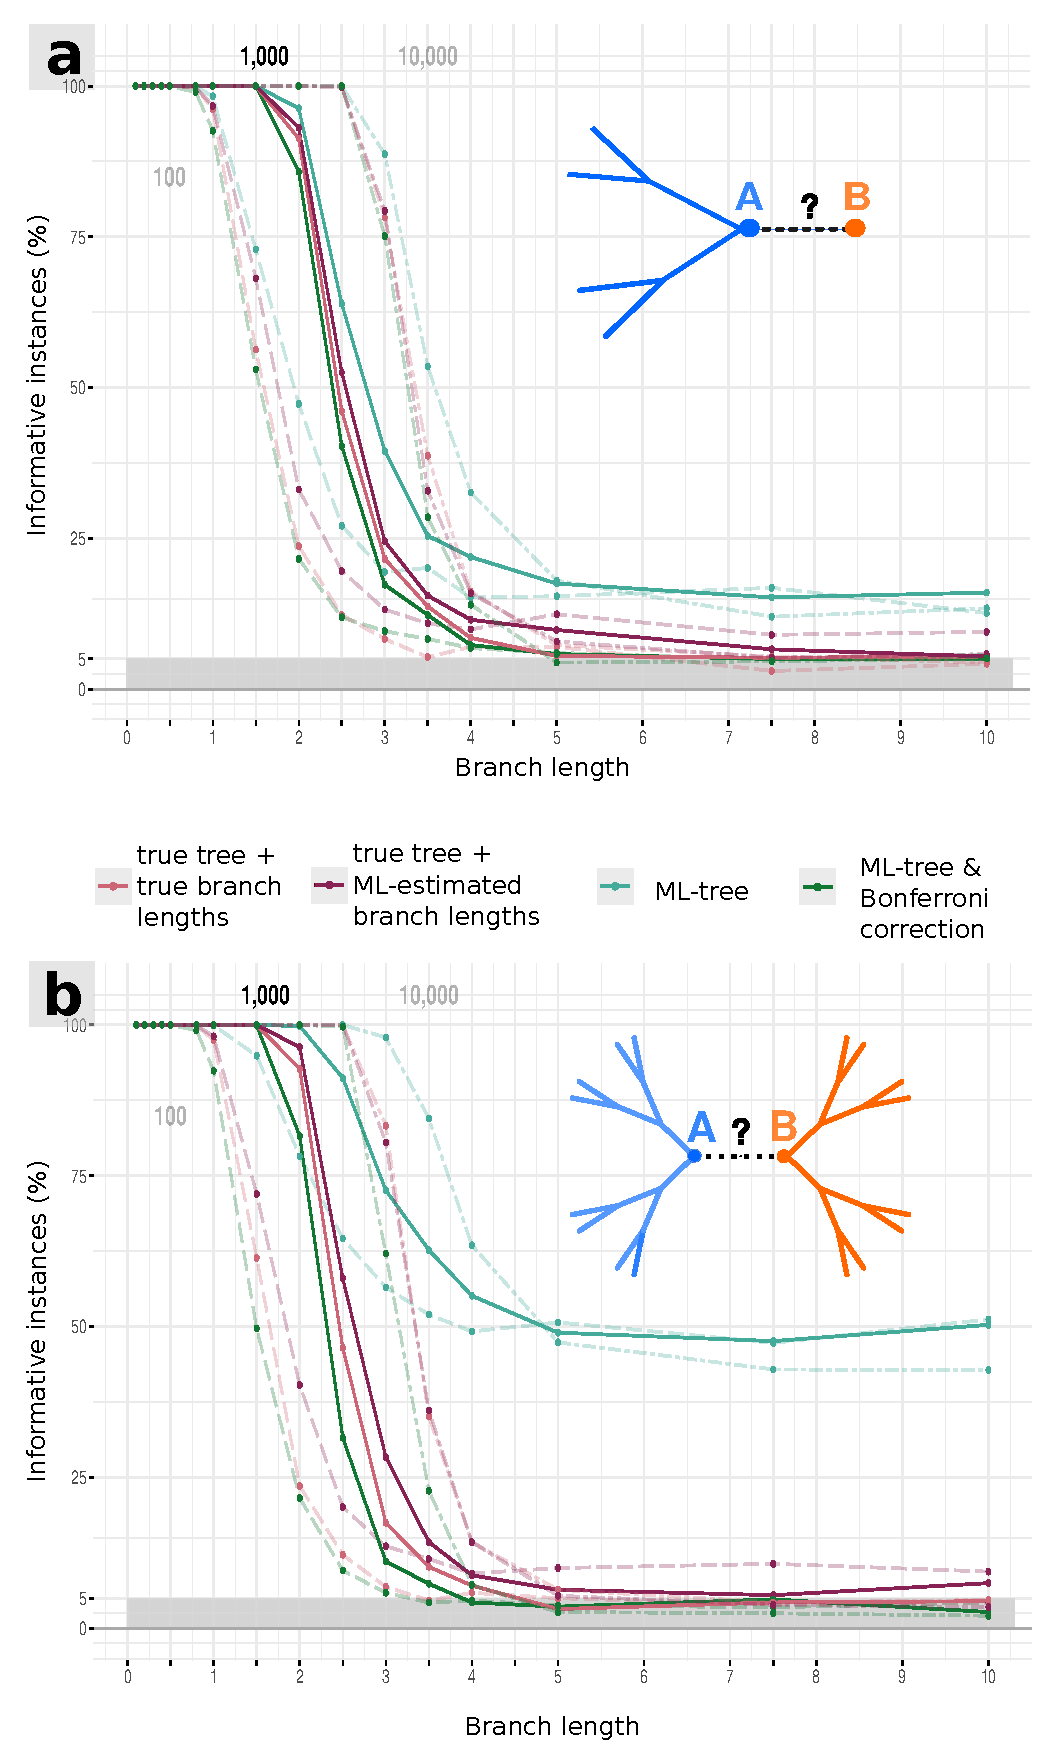
\includegraphics[width=0.82\textwidth]{figures/original/figure_simulated_data_main.pdf}
  \caption{\textbf{Original SatuTe simulation figure used as the reproduction target.} The extension analysis uses the same plotting structure: two tree cases, four analysis scenarios, three sequence lengths and the same branch-length grid. The figure is copied from the manuscript archive and is not regenerated from the local development output.}
\end{figure}

\begin{figure}[htbp]
  \centering
  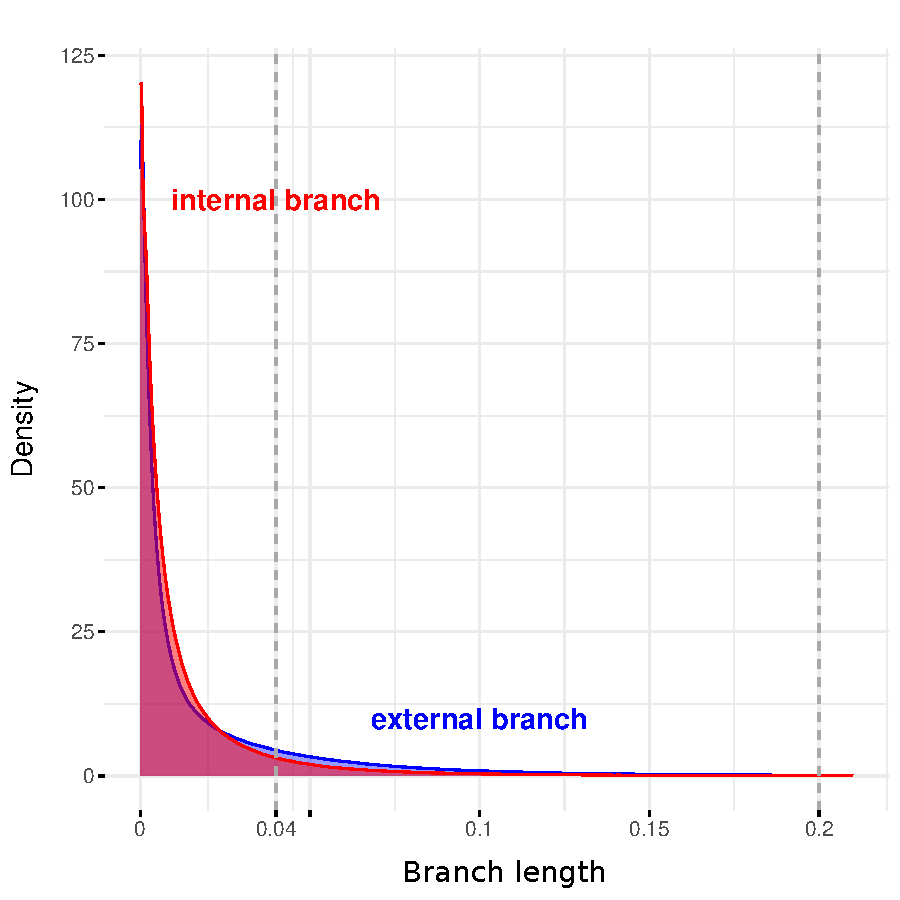
\includegraphics[width=0.55\textwidth]{figures/original/EvoNAPS_branch_length_distribution.pdf}
  \caption{\textbf{EvoNAPS branch-length distribution required for the 16-taxon simulations.} A direct rerun samples internal and external subtree branches from the empirical pools represented here. Fixed 0.1 subtree branches are used only for software development checks.}
\end{figure}

\subsection*{Validation must match the original simulation design}

The empirical comparison cannot be based on a small reduced run. A reduced run can test software wiring, branch selection and file parsing, but it cannot support claims about power, calibration or trustworthiness. The validation for this extension therefore starts by reproducing the SatuTe simulation design before adding GTR alternatives. In the JC baseline, branch length \(AB\) varies over \(\{0.1,0.2,0.3,0.4,0.5,0.8,1.0,1.5,2.0,2.5,3.0,3.5,4.0,5.0,7.5,10.0\}\), with \(1{,}000\) alignments per parameter combination and sequence lengths \(n=100,1{,}000,10{,}000\). The five-taxon case uses the \(B\mid A_1,A_2,A_3,A_4\) split described in the manuscript archive. The 16-taxon case uses the central \(A_1,\ldots,A_8\mid B_1,\ldots,B_8\) split with subtree branch lengths sampled from the EvoNAPS empirical distributions.

After the JC baseline reproduces the published behavior, the extension can be evaluated under GTR. The comparison is paired. One simulated alignment, one random seed, one analysis scenario and one target branch define a replicate. On that same replicate, the analysis computes the published dominant coefficient \(C_{\partial 1}\), the unweighted all-mode coefficient \(C_{\partial}^{\mathrm{all}}\), and the eigenvalue-weighted coefficient \(C_{\partial}^{\lambda}(t)\). The same one-sided normal test, the same \(\alpha\), and the same \(m_A m_B\) Bonferroni threshold are then applied to all three statistics. The endpoints are type I error under subtree independence, power under known informative branches, behavior under maximum-likelihood branch-length estimation, and inflation under maximum-likelihood topology selection with and without the Bonferroni correction.

The paired design changes the reporting. Power curves still show the fraction of replicates called informative, but each parameter combination should also include a discordance table: dominant-only, all-mode-only, weighted-only, all-mode versus weighted disagreements, and all formulas agreeing. McNemar tests on paired decisions and paired summaries of \(Z_{\lambda}(t)-Z_1\) or \(-\log_{10}P_{\lambda}+\log_{10}P_1\) compare formulas on the same simulated alignments and remove simulation noise shared by all formulas.

\begin{table}[htbp]
  \centering
  \caption{\textbf{Validation grid required for empirical claims.} The reduced files in this repository are development checks. They are not simulation evidence for power or calibration.}
  \small
  \begin{tabular}{p{0.22\textwidth}p{0.31\textwidth}p{0.35\textwidth}}
    \toprule
    Component & JC baseline & GTR enhancement \\
    \midrule
    Tree cases & Five-taxon external; 16-taxon internal & Same tree cases \\
    Branch lengths & Published 16-value grid & Same grid \\
    Sequence lengths & \(100,1{,}000,10{,}000\) & Same lengths \\
    Replicates & \(1{,}000\) per combination & \(1{,}000\) per combination \\
    Simulator & Seq-Gen-compatible JC design & GTR matrices with controlled spectra \\
    Scenarios & True fixed, true ML lengths, ML tree, Bonferroni & Same scenarios \\
    Replicate unit & One alignment, one scenario, one target branch & Same replicate for every formula \\
    Test threshold & Same \(\alpha\), same Bonferroni rule & Same \(\alpha\), same Bonferroni rule \\
    Statistics & \(C_{\partial 1}\) & \(C_{\partial 1}\), \(C_{\partial}^{\mathrm{all}}\), \(C_{\partial}^{\lambda}(t)\) \\
    Main comparison & Calibration of SatuTe baseline & Paired decisions and paired \(Z\)-score differences \\
    \bottomrule
  \end{tabular}
\end{table}

\section*{Discussion}

The extension changes the spectral aggregation step while keeping the SatuTe null test. SatuTe already derives branch saturation from the spectral decomposition of \(\operatorname{Diag}(\pi)P(t)\). The weighted statistic asks whether the coefficient tested by SatuTe should remain restricted to the single slowest mode under GTR, or whether other model-defined directions should contribute according to their expected persistence over branch \(AB\). Because the formula is built from \(C_{\partial i}\), \(\lambda_i\), \(\hat\sigma_{A,i,j}^{2}\), \(\hat\sigma_{B,i,j}^{2}\) and \(Z\), it keeps the notation and null logic of the original method.

This distinction can be framed as a calibration problem. The published \(C_{\partial 1}\) statistic is stringent in GTR because it tests only the slowest surviving non-stationary direction. The unweighted all-mode statistic is less stringent because it allows any spectral direction to contribute equally. The eigenvalue-weighted statistic allows all eigenvectors to contribute, but scales each contribution by the decay rate implied by the fitted model. On long branches, this makes the method approach the dominant SatuTe statistic. On short branches, non-dominant directions can still contribute.

The method is an extension rather than a replacement. The dominant SatuTe coefficient remains the reference statistic for branch saturation in IQ-TREE until the weighted statistic has been calibrated under the full simulation grid. If calibration supports the weighted test, it would add a model-aware diagnostic: not only whether two subtrees agree, but whether they agree in spectral directions that the fitted substitution model predicts should remain visible across the focal branch.

\section*{Online Methods}

\subsection*{Notation}

The notation follows SatuTe. A branch \(AB\) separates subtrees \(T_A\) and \(T_B\). A site pattern \(\partial\) induces subpatterns \(\partial_A\) and \(\partial_B\). The partial likelihood vectors at the endpoints are \(L(\partial_A)\) and \(L(\partial_B)\). The stationary distribution is \(\pi\), and \(P(\partial_A)=\langle L(\partial_A),\pi\rangle\), \(P(\partial_B)=\langle L(\partial_B),\pi\rangle\). The reversible rate matrix has eigenvalues \(\lambda_0=0>\lambda_1\geq\lambda_2\geq\lambda_3\) and left eigenvectors \(h_i\). Coherence coefficients are defined by \cref{eq-coherence}.

\subsection*{Weighted estimator}

For each site \(s\), compute \(C_{\partial_s i}\) for all non-stationary modes. For branch length \(t\), compute \(w_i(t)=\exp\{(\lambda_i-\lambda_1)t\}\). Then compute \(\hat C_{\lambda}(t)\), \(\hat\sigma_{\lambda}^{2}(t)\) and \(Z_{\lambda}(t)\) using \cref{eq-weighted-mean,eq-weighted-variance,eq-weighted-z}. If a model has a repeated second largest eigenvalue, all modes in that eigenspace have weight one. For JC, this gives the published SatuTe statistic.

\subsection*{Simulation protocol}

The baseline simulation first reproduces the published JC design. DNA alignments are generated with Seq-Gen, using the same tree cases, branch-length grid, sequence lengths and replicate count used for SatuTe. The five-taxon tree is a balanced four-taxon subtree \(T_A\) with all subtree branches set to 0.2 and a single taxon \(B\) attached by branch \(AB\). The 16-taxon tree is built from two balanced eight-taxon subtrees whose internal and external branch lengths are sampled from EvoNAPS-derived pools in the interval 0.04 to 0.2. Each alignment is analyzed under four scenarios: the true simulation tree with fixed true branch lengths, the true topology with maximum-likelihood branch lengths, the maximum-likelihood inferred tree, and the maximum-likelihood inferred tree with Bonferroni threshold \( \alpha/(m_A m_B) \). The GTR extension then repeats the same topologies and scenario logic with rate matrices chosen to span weak, moderate and strong separation between \(\lambda_1\), \(\lambda_2\) and \(\lambda_3\). Within each replicate, all formulas are evaluated on the same inferred or supplied tree, the same estimated branch length and the same target split.

\subsection*{Implementation status}

The local rerun script implements the paired design and the paper topologies. It records the simulator, branch-length source, target split, scenario, formula, \(Z\)-score, \(P\)-value and decision for every replicate. The script supports a direct rerun mode with Seq-Gen and an external EvoNAPS branch-length table, and a development-check mode using IQ-TREE AliSim with fixed 0.1 subtree branches when the raw EvoNAPS branch-length pools are not available. The development-check mode tests the IQ-TREE integration and formula comparison, but it is not evidence for the manuscript claims.

An exact rerun still requires three external inputs that are not present in the manuscript archive: the Seq-Gen binary, the raw EvoNAPS internal and external branch-length samples used for the 16-taxon simulations, and TreeShredder or an equivalent split-checking procedure to discard maximum-likelihood trees that do not recover the \(AB\) split. Without these dependencies, a run can verify code wiring but cannot claim to reproduce the original SatuTe simulation curves.

\section*{Data availability}

No full-scale simulation data are reported in this draft. The SatuTe source paper, the manuscript archive and public repositories are available from the cited sources. The local repository contains reduced outputs used only to verify command wiring, branch selection and paired formula evaluation.

\section*{Code availability}

The working IQ-TREE integration and manuscript sources are in the local repository. A publication version should archive the exact simulation scripts, IQ-TREE commit, SatuTe command lines, random seeds and generated summary tables.

\section*{Acknowledgements}

This manuscript draft builds on the SatuTe framework of Manuel and colleagues and on the IQ-TREE integration work in this repository.

\section*{Author contributions}

B.S. developed the enhancement concept and prepared the manuscript draft.

\section*{Competing interests}

The author declares no competing interests in this draft.

\begin{thebibliography}{9}

\bibitem{manuel2025satute}
Manuel, C., Sakalli, E., Schmidt, H. A., Viñas, C., von Haeseler, A. \& Elgert, C. When the past fades: detecting phylogenetic signal with SatuTe. \emph{Mol. Biol. Evol.} \textbf{42}, msaf090 (2025).

\bibitem{minh2020iqtree}
Minh, B. Q. et al. IQ-TREE 2: new models and efficient methods for phylogenetic inference in the genomic era. \emph{Mol. Biol. Evol.} \textbf{37}, 1530--1534 (2020).

\bibitem{rambaut1997seqgen}
Rambaut, A. \& Grassly, N. C. Seq-Gen: an application for the Monte Carlo simulation of DNA sequence evolution along phylogenetic trees. \emph{Bioinformatics} \textbf{13}, 235--238 (1997).

\bibitem{tavare1986}
Tavaré, S. Some probabilistic and statistical problems in the analysis of DNA sequences. \emph{Lect. Math. Life Sci.} \textbf{17}, 57--86 (1986).

\bibitem{levin2017}
Levin, D. A. \& Peres, Y. \emph{Markov Chains and Mixing Times}. 2nd edn. American Mathematical Society (2017).

\end{thebibliography}

\end{document}
